%!TEX root = slides.tex
% Добавьте ссылку на файлы с текстом работы
% Можно использовать команды:
%   \input или \include
% Пример:
%    \input{mainfiles/1-section} или \include{mainfiles/2-section}
% Команда \input позволяет включить текст файла без дополнительной обработки
% Команда \include при включении файла добавляет до него и после него команду
% перехода на новую страницу. Кроме того, она позволяет компилировать каждый файл
% в отдельности, что ускоряет сборку проекта.
% ВАЖНО: команда \include не поддерживает включение файлов, в которых уже содержится команда \include,
% т.е. не возможен рекурсивный вызов \include
\newcommand*{\Source}{
    %!TEX root = ../slides.tex

\section{Глиальные опухоли}

\begin{frame}
  \frametitle{Глиальные опухоли}
  %\framesubtitle{Subtitles are optional.}
  % - A title should summarize the slide in an understandable fashion
  %   for anyone how does not follow everything on the slide itself.

  \begin{itemize}
  \item
  Глиальная опухоль является патологическим новообразованием, расположенным внутри мозга. 
  Она развивается из глии – вспомогательных клеток нервной ткани.
  
  \item
  Согласно классификации ВОЗ, глиальные опухоли делятся на четыре типа. В основе этой классификации лежит 4 основных признака:
    \begin{itemize}
      \item атипия клетки
      \item фигуры митозов
      \item наличие области некроза (отмирания тканей)
      \item разрастание эндотелия
    \end{itemize}
    
  \item Глиомы бывают:
    \begin{itemize}
      \item доброкачественными
      \item злокачественными
    \end{itemize}
     
  \end{itemize}
\end{frame}

\subsection{Методы обследования глиальных опухолей}

\begin{frame}
  \begin{itemize}
    \frametitle{Методы обследования глиальных опухолей}
    \item Компьютерная томография с контрастным усилением (КТ)
    \item Магнитно-резонансная томография  с контрастным усилением (МРТ)
    \item ПЭТ 
    \item Сцинтиграфия
    \item Неврологическое исследование, которое обязательно включает в себя офтальмологическую проверку остроты зрения, глазного дна и полей зрения
    \item Ангиография
  \end{itemize}
\end{frame}
    %!TEX root = ../slides.tex
\section{Актуальность}
\begin{frame}
    \frametitle{Актуальность}
    \begin{itemize}
        \item Число глиом составляет более 60 \% от всех опухолей центральной нервной системы.
        мозга.
        \item Ранняя диагностика опухоли способствует высоким результатам лечения. Заболевание нуждается в дифференцировке от 
        гематомы внутри мозга, абсцесса, эпилепсии, прочих опухолевых процессов в центральной нервной 
        системе, последствий инсульта.
        \item Автоматическая сегментация/классификация глиальных опухолей головного мозга по ПЭТ-изображениям
        ускорит процесс дифференциальной диагностики и поможет определить вектор последующих исследований и лечения.
        
    \end{itemize}
\end{frame}

\section{Цель}
\begin{frame}
    \frametitle{Цель}
    \begin{itemize}
        \item Разработать метод искусственного интеллекта \(F\), который по 
        данным из обучающей выборки \(X={x_1,\dots,x_n}\),
        состоящей из ПЭТ-изображений, возвращает результат предсказания \(y=F(X)\), 
        где y - это бинарный признак наличия опухоли либо степень ее опасности.
    \end{itemize}
\end{frame}

\section{Постановка задачи}
\begin{frame}
    \frametitle{Постановка задачи}
    \begin{itemize}
        \item Сделать обзор существующих методов классификации и сегментации опухолей головного мозга,
        визуализирующихся на ПЭТ-изображениях.
        \item Найти и скомпилировать датасет, на которых будет производиться исследование.
        \item На полученном датасете применить методы сегментации/классификации из обзора, 
        сравнить результаты.
        \item Разработать собственный метод для улучшения процесса дифференциальной 
        диагностики глиальных опухолей.
        \item Провести эксперименты с полученным решением.
    \end{itemize}
\end{frame}
    %!TEX root = ../slides.tex
\section{ПЭТ - исследование}
\begin{frame}
    \frametitle{ПЭТ - исследование}
    \begin{itemize}
        \item Позитронно-эмиссионная томография (ПЭТ) — технология 
        визуализации, основанная на количественной и качественной 
        оценке биохимических процессов, происходящих в тканях \textit{in vivo}.
    \end{itemize}
\end{frame}
\subsection{Принцип работы ПЭТ}
\begin{frame}
    \frametitle{Принцип работы ПЭТ}
    \begin{figure}
        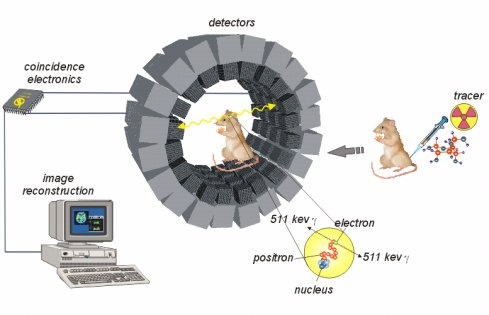
\includegraphics[scale=0.5]{pet.jpg}
    \end{figure}

    \begin{itemize}
        \item Как отличить здоровую ткань от «нездоровой»?
    \end{itemize}
    \[SUV_{\chi}=\frac{C(t)}{D/\chi}\]
\end{frame}


\begin{frame}
    \frametitle{Примеры ПЭТ - изображений}

    \begin{figure}[htbp]
        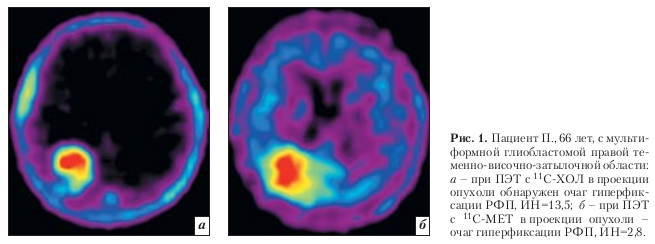
\includegraphics[scale=0.3]{pet_ex1.png}
        \hfill
        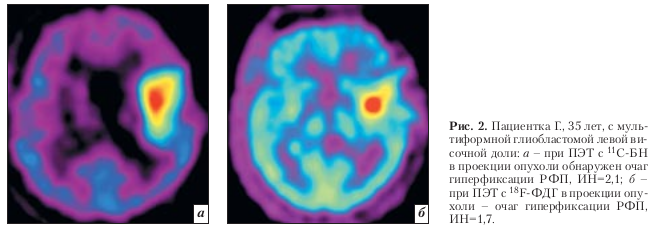
\includegraphics[scale=0.3]{pet_ex2.png}   
    \end{figure}

    \begin{figure}
        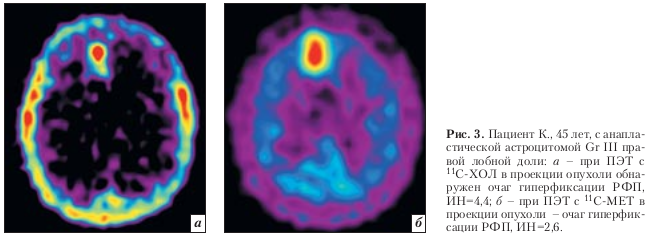
\includegraphics[scale=0.3]{pet_ex3.png}
    \end{figure}
\end{frame}

\subsection{ПЭТ/КТ, ПЭТ/МРТ}
\begin{frame}
    \frametitle{КТ, МРТ}
    \begin{itemize}
        \item Компьютерная томография (КТ) - это специальный метод визуализации, в котором используется рентгеновское излучение. 
        \item Магнитно-резонансная томография (МРТ) - метод визуализации, основанный на резонансе атомов водорода в организме человека на магнитное поле, 
        создаваемое томографом.
    \end{itemize}
    \begin{figure}[htbp]
        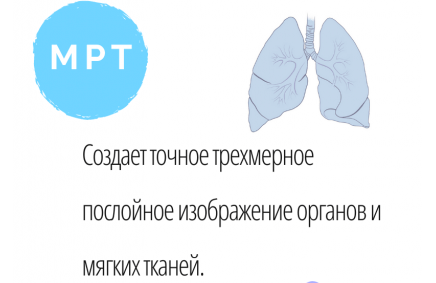
\includegraphics[scale=0.35]{mri.png}
        \hfill
        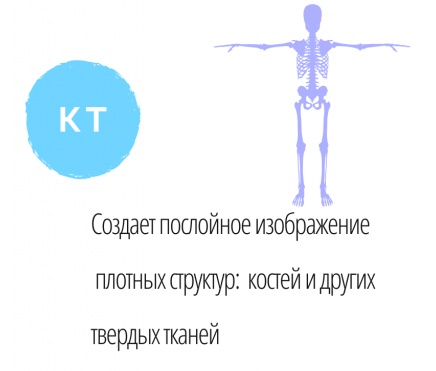
\includegraphics[scale=0.35]{ct.png}
    \end{figure}
\end{frame}

\begin{frame}
    \frametitle{ПЭТ/КТ, ПЭТ/МРТ}
    \begin{figure}
        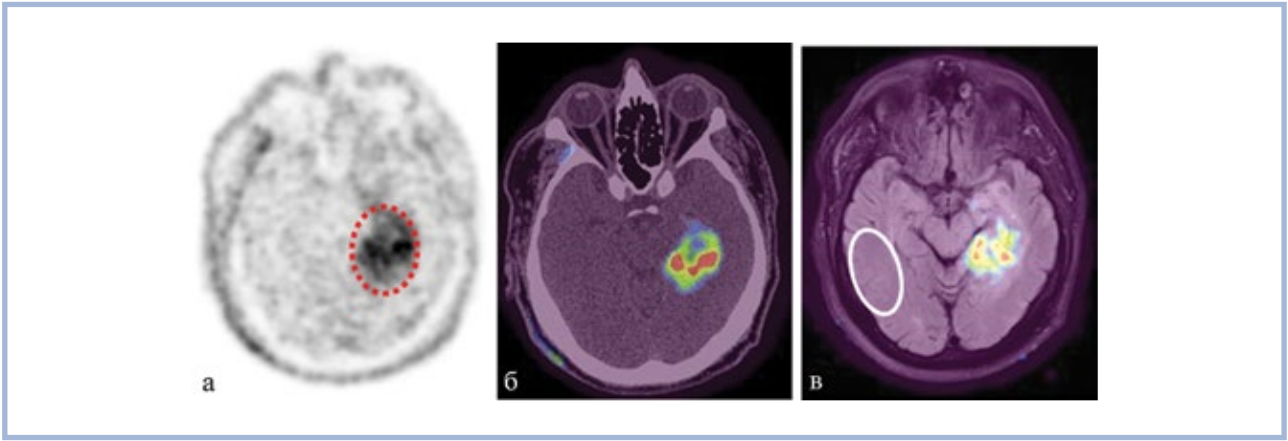
\includegraphics[scale=0.3]{pet_mri_ct.png}
    \end{figure}
\end{frame}
    %!TEX root = ../slides.tex
\section{Методы сегментации ПЭТ изображений}
\begin{frame}
    \frametitle{Методы сегментации ПЭТ изображений. Общая информация}
    \begin{itemize}
        \item Без ограничения общности, сегментацию изображений
        можно представлять как две связанные задачи:
        \textit{распознавание} и \textit{оконтуривание}.
        \item Внешние и внутренние факторы, значительно
         влияющие на сегментацию ПЭТ-изображений:
         \begin{itemize}
             \item проблемы, связанные с разрешением изображения
             \item многовариантность форм, текстуры и расположения патологий
             \item шум
         \end{itemize}
        
    \end{itemize}
\end{frame}

\begin{frame}
    \frametitle{Методы}
    \begin{figure}
        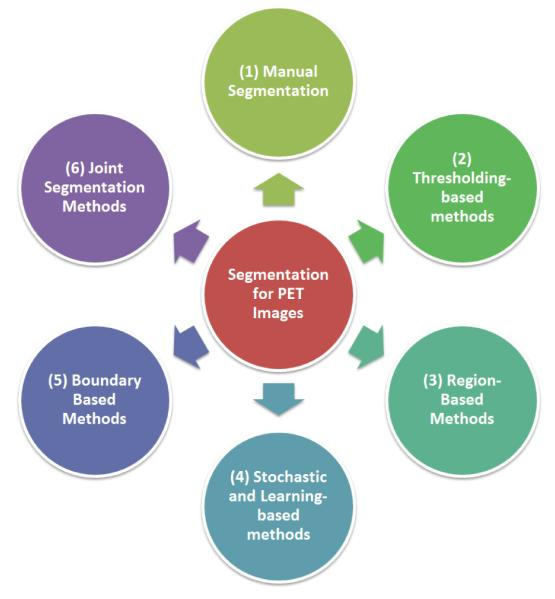
\includegraphics[scale=0.8]{cluster.jpg}
    \end{figure}
\end{frame}

%\subsection{Ручная сегментация}
%\begin{frame}
 %   \frametitle{Ручная сегментация}
  %  \begin{itemize}
   %     \item Конструирование размеченного множества изображений (ground truth)
    %    \item Оценка качества 
     %  \[DSC(V_1, V_2) = 2\frac{|V_1\cup V_2|}{|V_1|+|V_2|}\]
      % \item Сложности         
    %\end{itemize}
%\end{frame}

\subsection{Пороговые методы}
\begin{frame}
    \frametitle{Пороговые методы}
    \begin{itemize}
        \item Простой, интуитивно понятный и популярный метод,
        при котором черно-белое изображение конвертируется в бинарное, и пиксели больше определенного 
        значения считаются передним планом, а меньше - фоном.
        \item Сложность - определить оптимальное пороговое значение.        
    \end{itemize}
\end{frame}
\subsection{Стохастические модели и модели, основанные на обучении}
\begin{frame}
    \frametitle{Стохастические модели и модели, основанные на обучении}
    \begin{itemize}
        \item \textit{Mixture models} - объекты на ПЭТ-изображении
        имеют примерно гауссовское распределение и это априорное знание 
        может помочь в сегментации.
        \item \textit{Fuzzy locally adaptive Bayesian (FLAB) method} - статистический
        unsupervised метод, при котором считается, что изображение содержит два класса твердых
        тканей и конечное число \grqq нечетких уровней\glqq, которые 
        включают в себя смесь двух классов. Из-за свойства нечеткости 
        воксели принадлежат одному из двух классов, а уровень их 
        \grqq нечеткости\glqq определяется степенью принадлежности к каждому из классов.
        \item \textit{Clustering/Classification of PET image intensities}
        \begin{itemize}
            \item Классификация - разделение пространства объектов, полученного из изображения, с помощью известных меток
            \item Кластеризация - используется пространственная информацию, содержащаяся в изображениях, но без использования обучающих данных
        \end{itemize}
    \end{itemize}
\end{frame}

\subsection{Методы сегментации, основанные на регионах}
\begin{frame}
    \frametitle{Методы сегментации, основанные на регионах}
    Сегментация на основе регионов, в которых однородность 
    изображения является основным фактором для определения 
    границ объекта.
    \begin{itemize}
        \item \textit{Region Growing} - метод, который включает пространственную информацию в изображение наряду с информацией об интенсивности.
        \item \text{Графовые методы}
        \begin{itemize}
            \item Graph-cut
            \item Random walk

        \end{itemize}
        
    \end{itemize}
    
\end{frame}
\subsection{Методы выделения границ}
\begin{frame}
    \frametitle{Методы выделения границ}
    \begin{itemize}
        \item \textit{Active Contours (snakes)} - начальный контур 
        вокруг интересующего объекта деформируется и движется к желаемым границам.
        \item \textit{Level Set} - способ моделирования активных контуров путем отслеживания 
        границ между различными фазами потоков жидкости.
        \item \textit{Градиентные методы} - обычно, на границе происходит резкое изменение значения интенсивности. 
        Чтобы определить, где это происходит, вычисляется градиент между рассматриваемым вокселем и его соседями.
    \end{itemize}
\end{frame}

\subsection{Совместная сегментация}
\begin{frame}
    \frametitle{Совместная сегментация}
    \begin{itemize}
        \item Для сегментации совмещаются несколько изображений различных модальностей, 
        содержащих дополнительную информацию из входных данных. Обычно это ПЭТ/КТ и ПЭТ/МРТ.
    \end{itemize}
\end{frame}    
    %\include{mainfiles/2-mceliece-sidelnikov}
    %%!TEX root = ../annotations.tex

\section{Ключевое пространство криптосистемы Мак-Элиса.}
В исследованиях криптосистем с открытым ключом возникает вопрос о
числе  открытых ключей, так как некоторые разные секретные ключи
могут порождать одинаковые открытые ключи. Если этих ключей
достаточно мало, то злоумышленник сможет эффективно строить по
открытому ключу некоторого легального абонента свой секретный
ключ. Что даст ему возможность читать все секретные сообщения,
приходящие в адрес абонента. Идеально, когда в криптосистеме любые
два различных секретных ключа порождают неравные друг другу
открытые ключи. Однако, часто в кодовых криптосистемах это не так.
В связи с чем возникает естественный вопрос, а сколько всего
открытых ключей.

Везде в этом параграфе предполагается, что в криптосистеме
Мак-Элиса в качестве порождающей матрицы кода $\mathcal C$ была
выбрана матрица $G$, а сам код имеет длину равную $n$, размерность
--- $k$ и кодовое расстояние --- $d$.  Легальный абонент в
качестве своего секретного ключа выбрал тройку $(H,G,\Gamma)$
(здесь $G$ включается в секретный ключ для удобства, на самом
деле, $G$ --- общедоступная матрица, выбираемая заранее), тогда
соответствующий открытый ключ будет равен произведению этих матриц
$H\cdot G\cdot \Gamma$. Введём отношение эквивалентности секретных
ключей следующим способом \Def{Два секретных ключа
$(H',G,\Gamma')$ и $(H'',G,\Gamma'')$ назовём
\emph{эквивалентными}, если и только если выполняется соотношение
$$
H'\cdot G\cdot\Gamma'=H''\cdot G\cdot\Gamma'',
$$
то есть порождаемые ими открытые ключи совпадают.}

Легко видеть, что данное отношение --- отношение эквивалентности.
Тем самым всё множество секретных ключей разбивается на классы
эквивалентности. В дальнейшем класс с представителем
$(H,G,\Gamma)$ будем обозначать как $[(H,G,\Gamma)]$

Важную роль в исследовании классов эквивалентности
$[(H,G,\Gamma)]$ играет группа автоморфизмов кода $\mathcal C$,
напомним ее определение.

\Def{\label{opr1}\emph{Группой автоморфизмов} кода $\mathcal C$
называется множество
$$
Aut(\mathcal C)=\{\Gamma\in S_n|\exists\; A\in GL_k(F_q):
G\Gamma=AG\},
$$
где $S_n$ --- симметрическая группа степени $n$, $GL_k(F_q)$ ---
группа всех невырожденных $k\times k$-матриц над полем $F_q$, а
перестановка $\Gamma\in S_n$ представляется перестановочной
$k\times k$-матрицей, которая действует на $G$ как соответствующая
перестановка столбцов. }

 С группой автоморфизмов неразрывно связано множество $\mathcal
A(\mathcal C)$ невырожденных $k\times k$-матриц, задающих
перестановки из группы автоморфизмов, то есть
$$
\mathcal A(\mathcal C)=\{A\in GL_k(F_q)|\exists\; \Gamma\in
Aut(G): AG=G\Gamma\}.
$$
\begin{proposition}
Пусть кодовое расстояние кода $\mathcal C^{\perp}$, дуального к
коду $\mathcal C$, строго больше двух. Тогда для любой матрицы
$A\in GL_k(F_q)$, принадлежащей множеству $\mathcal A(\mathcal
C)$, существует и единственная перестановка $\Gamma$ из группы
автоморфизмов $Aut(\mathcal C)$. И для любой перестановки
$\Gamma\in Aut(\mathcal C)$ существует и единственная матрица
$A\in\mathcal A(\mathcal C)$.
\end{proposition}
\begin{proof}
Пусть $A$ принадлежит $\mathcal A(\mathcal C)$, тогда найдётся
перестановка $\Gamma$ такая, что
$$
AG=G\Gamma.
$$
Очевидно, что $\Gamma\in Aut(\mathcal C)$. Докажем, что такая
$\Gamma$ единственна. Пусть существуют две перестановки $\Gamma'$
и $\Gamma''$ такие, что
$$
AG=G\Gamma'\;\;\;AG=G\Gamma''.
$$
Тогда
$$
G\Gamma'\Gamma''^{-1}=G.
$$
В силу того, что кодовое расстояние $\mathcal C^{\perp}$ строго
больше двух, то в матрице $G$ нет двух одинаковых столбцов.
Поэтому из последнего соотношения следует, что
$$
\Gamma'\Gamma''^{-1}=E.
$$
Полученное соотношение, означает, что $\Gamma'=\Gamma''$.

Докажем, что для $\Gamma\in Aut(\mathcal C)$ найдётся единственная
матрица $A\in \mathcal A(\mathcal C).$ В силу того, что $\Gamma\in
Aut(\mathcal C)$, то существует $A$, с которой
$$
AG=G\Gamma.
$$
Понятно, что $A\in\mathcal A(\mathcal C)$. Если найдутся две
матрицы $A'$ и $A''$ такие, что
$$
A'G=G\Gamma\;\;A''G=G\Gamma,
$$
то $A'G=A''G$. Ранг матрицы $G$ равен $k$, поэтому $A'=A''$.

Утверждение полностью доказано.
\end{proof}

Известно следующее утверждение, устанавливающее связь между
группой автоморфизмов кода $\mathcal C$ с порождающей матрицей $G$
и эквивалентными ключами криптосистемы Мак-Элиса.
\begin{proposition}\label{prop4}
Пусть в качестве порождающей матрицы кода $\mathcal C$ в
криптосистеме Мак-Элиса взята матрица $G$. Тогда существует
взаимно однозначное соответствие между множеством $Aut(\mathcal
C)$ и классом эквивалентности $[(H,G,\Gamma)]$ множества секретных
ключей криптосистемы Мак-Элиса.
\end{proposition}
\begin{proof}
Действительно, поставим секретному ключу
$(H',G,\Gamma')\in [(H,G,\Gamma)]$ в соответствие перестановку
$\Gamma'\Gamma^{-1}$. Докажем, что это перестановка принадлежит
группе автоморфизмов кода $\mathcal C$. В силу того, что
$(H',G,\Gamma')$ принадлежит классу $[(H,G,\Gamma)]$, то
выполняется соотношение
$$
HG\Gamma=H'G\Gamma'.
$$
Умножая правую и левую его части справа на матрицу $\Gamma^{-1}$, а
слева на $H'^{-1}$, получаем, что для перестановки
$\Gamma'\Gamma^{-1}$ справедливо соотношение
$$
H'^{-1}HG=G\Gamma'\Gamma^{-1}.
$$
Последнее и означает, что $\Gamma'\Gamma^{-1}$ принадлежит группе
автоморфизмов кода $\mathcal C$. Очевидно, данное  отображение
сюръективно. Покажем, что оно инъективно. Пусть существуют два
секретных ключа $(H',G,\Gamma')$ и  $(H'',G,\Gamma'')$ из класса
эквивалентности $[(H,G,\Gamma)]$, для которых
$\Gamma'\Gamma^{-1}=\Gamma''\Gamma^{-1}$. Тогда,
$\Gamma'=\Gamma''$. И, так как $H'G\Gamma'=H''G\Gamma''$, то равны
матрицы $H'$ и $H''$. Из всего сказанного следует, что ключи
$(H',G,\Gamma')$ и $(H'',G,\Gamma'')$ совпадают.

Утверждение полностью доказано.
\end{proof}

\begin{proposition}
Класс эквивалентности $[(H,G,\Gamma)]$ состоит из всех троек вида
$(H\cdot D_{\Gamma_A},G,\Gamma^{-1}_A\cdot \Gamma)$, где
$\Gamma_A\in Aut(\mathcal C)$, а $D_{\Gamma_A}G=G\Gamma_A$.
\end{proposition}
\begin{proof}
При доказательстве утверждения~\ref{prop4} было получено, что для
любого элемента $(H',G,\Gamma')\in[(H,G,\Gamma)]$ матрица
$H'^{-1}H$ принадлежит множеству $\mathcal A(\mathcal C)$, а
$\Gamma'\Gamma^{-1}$ --- соответствующая перестановка из группы
автоморфизмов кода $\mathcal C$, то есть $\Gamma'\Gamma^{-1}\in
Aut(\mathcal C)$. Если теперь положить $D_{\Gamma_A}=H'^{-1}H$ и
$\Gamma_A=\Gamma'\Gamma^{-1}$, то получим требуемое.
\end{proof}

Из этого утверждения немедленно получаем формулу для мощности
множества открытых ключей, которая совпадает с числом классов
эквивалентности секретных ключей.

\begin{proposition}\label{prop5}
Пусть $\mathcal E$ --- множество всех открытых ключей
криптосистемы Мак--Элиса. Тогда справедлива формула
$$
|\mathcal E|=\frac{n!h_k(q)}{|Aut(\mathcal C)|},
$$
здесь $h_k(q)=|GL_k(F_q)|=(q^k-1)(q^k-q)\ldots (q^k-q^{k-1})$ ---
число невырожденных матриц порядка $k$ над полем $F_q$.
\end{proposition}
\begin{proof}
Из утверждения~\ref{prop4} следует, что каждый класс
эквивалентности состоит из одного и того же числа элементов, а
именно из $|Aut(\mathcal C)|$ элементов, поэтому число классов, а
значит и число открытых ключей, будет равно отношению общего числа
секретных ключей к мощности класса эквивалентности. Всего
секретных ключей столько сколько пар $(H,\Gamma)$, где $H$
--- невырожденная $k\times k$-матрица, а $\Gamma$ ---
перестановочная $n\times n$-матрица. Число матриц $H$ равно
$h_k(q)$, а число всех перестановок --- $n!$, поэтому общее число
пар $(H,\Gamma)$ в точности равно $n!h_k(q)$. Учитывая всё
сказанное, получаем требуемую формулу.
\end{proof}
Заметим, что формула утверждения~\ref{prop5} даёт также общее
число  классов эквивалентности секретных ключей криптосистемы
Мак-Элиса.

Тем самым вопрос изучения классов эквивалентности секретных ключей
криптосистемы Мак-Элиса сводится к известной и трудной задаче
теории кодирования
--- описание группы автоморфизмов кода.

Одним из примеров кодов, для которых полностью вычислена группа
автоморфизмов, является двоичный код Рида--Маллера $RM(r,m)$, см.\
например~\cite{McWilliams}. Его группа автоморфизмов
$Aut(RM(r,m))$ представляет из себя полную аффинную группу
пространства $F^m_2$. Мощность этой группы равна $2^mh_m(2)$.
Поэтому справедливо утверждение.

\begin{proposition}
Общее число открытых ключей в криптосистеме Мак-Элиса, в которой в
качестве матрицы $G$ была выбрана порождающая матрица двоичного
кода Рида--Маллера, вычисляется по формуле
$$
|\mathcal E|=\frac{n!h_k}{2^mh_m},
$$
здесь $h_k=h_k(2)$ и $h_m=h_m(2)$.
\end{proposition}

Информацию о группах автоморфизмов других известных кодов можно
найти в~\cite{HandBook}.
    %\include{mainfiles/4-mceliece-sidelnikov-equivalence}
    %\include{mainfiles/5-restore-part-of-sec-key}
    %\include{mainfiles/6-conclude}
    %!TEX root = ../slides.tex

\section{План работ}
\begin{frame}
    \frametitle{План работ}
    \begin{itemize}
        \item На текущий семестр:
            \begin{itemize}
                \item Сделать обзор существующих методов классификации и сегментации опухолей головного мозга,
                визуализирующихся на ПЭТ-изображениях - \textbf{сделано}.
                \item Уточнить постановку задачи
            \end{itemize}
        \item В следующем семестре:
            \begin{itemize}
                \item Найти и скомпилировать датасет, на которых будет производиться исследование.
                \item На полученном датасете применить методы сегментации/классификации из обзора, 
                сравнить результаты.
            \end{itemize}
    \end{itemize}
\end{frame}

\begin{frame}
    \begin{center}
        \text{СПАСИБО ЗА ВНИМАНИЕ!}
    \end{center}
\end{frame}
    %%!TEX root = ../slides.tex

\section{Список литературы}

\begin{frame}
\frametitle{Список литературы}
\nocite{*}
%\begin{alertblock}{Из списка ВАК}
\printbibliography %[keyword=VAK, title=Из списка ВАК]
%\end{alertblock}
%\begin{exampleblock}{Другие}
%\printbibliography[keyword=NoVAK, title=Из списка ВАК]
%\end{exampleblock}
\end{frame}

}


% Информация о годе выполнения работы
\newcommand{\Date}{%
    % 16 июня 2010 г.%
    %\today%     % Текущий день
    17 ноября 2021 г.
}

% Укажите тип работы
% Например:
%     Выпускная квалификационная работа,
%     Магистерская диссертация,
%     Курсовая работа, реферат и т.п.
\newcommand{\WorkType}{%
    % Выпускная квалификационная работа%
    % Магистерская диссертация%
    Курсовая работа%
    % Реферат%
    %Доклад
}

% Название работы
%%%%%%%%%%% ВНИМАНИЕ! %%%%%%%%%%%%%%%%
% В МГУ ОНО ДОЛЖНО В ТОЧНОСТИ
% СООТВЕТСТВОВАТЬ ВЫПИСКЕ ИЗ ПРИКАЗА
% УТОЧНИТЕ НАЗВАНИЕ В УЧЕБНОЙ ЧАСТИ
\newcommand{\Title}{%
    Обзор методов дифференциальной диагностики глиальных опухолей по данным динамических ПЭТ - исследований%
}


% Имя автора работы
\newcommand{\Author}{%
    Айрапетьянц Каринэ Арсеновна%
}

% Информация о научном руководителе
%% Фамилия Имя Отчество%
\newcommand{\SciAdvisor}{%
    Малоян Нарек Гагикович%
}
%% В формате: И.~О.~Фамилия%
\newcommand{\SciAdvisorShort}{%
    Н.~Г.~Малоян%
}
%% должность научного руководителя
\newcommand{\Position}{%
    % профессор%
    %доцент
    % старший преподаватель%
    % преподаватель%
    % ассистент%
    % ведущий научный сотрудник%
    % старший научный сотрудник%
    % научный сотрудник%
    % младший научный сотрудник%
}
%% учёная степень научного руководителя
\newcommand{\AcademicDegree}{%
    % д.ф.-м.н.%
    % д.т.н.%
    %к.ф.-м.н.
    % к.т.н.%
    % без степени%
}

% Информация об организации, в которой выполнена работа
%% Город
\newcommand{\Place}{%
    Москва%
}
%% Университет
\newcommand{\Univer}{%
    Московский государственный университет имени М.~В.~Ломоносова%
}
\newcommand*{\UniverAbbr}{%
    МГУ%
}
%% Факультет
\newcommand{\Faculty}{%
    Факультет вычислительной математики и кибернетики%
}
%% Кафедра    
\newcommand{\Department}{%
    Кафедра информационной безопасности%
}     

%%%% Переключите формат экрана
\newcommand{\Aspect}{%
    % 43%
    % 1610%
    169%
}
